% Copyright (C) 2020 - Michael Baudin

% \documentclass{beamer}
\documentclass[aspectratio=169]{beamer}
%\setbeameroption{hide notes}
%\setbeameroption{show notes}
%\setbeameroption{show only notes}

% Copyright (C) 2012 - EDF R&D - Michael Baudin

% To highlight source code
\usepackage{listings}
\definecolor{darkgreen}{rgb}{0,0.5,0}
\definecolor{violet}{rgb}{0.5,0,1}

\usepackage{lmodern}% http://ctan.org/pkg/lm

\usetheme{Montpellier}
\setbeamertemplate{navigation symbols}{} % Remove navigation
\useoutertheme{infolines}

\usepackage[utf8]{inputenc}
\usepackage[T1]{fontenc}

%\usepackage[french]{babel}
%\uselanguage{French}
%\languagepath{French}

\def\bx{{\bf x}}
\def\RR{\mathbb{R}}

\newcommand{\pyvar}[1]{\texttt{#1}}

\def \ot {OpenTURNS}

\hypersetup{colorlinks=true}


\title[PERSALYS]{PERSALYS, the graphical interface of OpenTURNS}

\author[PERSALYS Team]{
M. Baudin \inst{1} \and
T. Delage \inst{1} \and
A. Dumas \inst{2} \and
A. Dutfoy \inst{1} \and \\
G. Garcia \inst{2} \and
A. Geay \inst{1} \and
O. Mircescu \inst{1} \and
J. Pelamatti \inst{1} \and \\
F. Robin \inst{1} \and
J. Schueller \inst{2} \and
T. Yalamas \inst{2}
}

\institute[EDF-Phimeca]{
\inst{1} EDF R\&D. 6, quai Watier, 78401, Chatou Cedex - France, michael.baudin@edf.fr \and %
\inst{2} Phimeca Engineering. 18/20 boulevard de Reuilly, 75012 Paris - France, yalamas@phimeca.com
}

\date[]{June 10th 2022, OpenTURNS User's day}

%%%%%%%%%%%%%%%%%%%%%%%%%%%%%%%%%%%%%%%%%%%%%%%%%%%%%%%%%%%%%%%%%%%%%%%%%%%%%

  \begin{document}

%%%%%%%%%%%%%%%%%%%%%%%%%%%%%%%%%%%%%%%%%%%%%%%%%%%%%%%%%%%%%%%%%%%%%%%%%%%%%

\begin{frame}
  \titlepage

  \begin{columns}
    \column{0.45\textwidth}
  \begin{center}

\includegraphics[height=0.15\textheight]{figures/edf.jpg}
\end{center}
    \column{0.1\textwidth}

    \column{0.45\textwidth}
  \begin{center}

\includegraphics[height=0.15\textheight]{figures/logo_phimeca.png}
\end{center}
  \end{columns}

\end{frame}

\note{
I would like to thank the organizers to inviting us to present our tools.
}

%%%%%%%%%%%%%%%%%%%%%%%%%%%%%%%%%%%%%%%%%%%%%%%%%%%%%%%%%%%%%%%%%%%%%%%%%%%%%

\begin{frame}
\frametitle{Contents}
\tableofcontents
\end{frame}

\section{Overview}

\begin{frame}
  \frametitle{Bring Uncertainty Methodology to Engineers}
  \begin{itemize}
  \item Partnership started in 2015

    \begin{itemize}
    \item EDF R\&D wanted to maximize the use of OpenTURNS\textregistered{} by its engineer/researcher (and improve an existing GUI) $\rightarrow$ develop a GUI to make more easy to use

    \item Phimeca had already developed an "OpenTURNS GUI" (PhimecaSoft\textregistered{}) which satisfies some needs of EDF R\&D but not all.

    \item EDF R\&D and Phimeca decided to start a specific partnership in order to develop a new GUI based on OpenTURNS\textregistered{} and "Salome Tools": Paraview, Yacs, ...
    \end{itemize}
  \end{itemize}
\end{frame}

%%%%%%%%%%%%%%%%%%%%%%%%%%%%%%%%%%%%%%%%%%%%%%%%%%%%%%%%%%%%%%%%%%%%%%%%%%%%%

\begin{frame}
  \frametitle{Some expectations regarding the GUI}
  \begin{itemize}
  \item As easy to use as possible and, when it is possible, a GUI which can guide the user

  \item Possibility to use it inside Salome Platform to
    \begin{itemize}
    \item Use supercomputing resources (e.g. Gaïa, 3 052 Tflops peak, 41 000 cores)
    \item Connect to EDF numerical code users (Code\_Aster for example)
    \end{itemize}

  \item Take benefit from the advanced visualization capability from Paraview

  \item Drive the GUI from a python script usable in an "expert" mode
  \end{itemize}
\end{frame}

%%%%%%%%%%%%%%%%%%%%%%%%%%%%%%%%%%%%%%%%%%%%%%%%%%%%%%%%%%%%%%%%%%%%%%%%%%%%%

\begin{frame}
  \frametitle{PERSALYS, the graphical user interface of \ot{}}

  \begin{itemize}
  \item Main goal : provide a graphical interface of
    \ot{} in the SALOME integration platform
  \item Features
    \begin{itemize}
    \item Uncertainty quantification : definition of the
      probabilistic model (including dependence), distribution fitting (including
      copulas), physical model with vector input
      and vector output or 1D Fields,
      central tendency, sensitivity analysis, probability estimate,
      metamodeling (polynomial chaos, kriging), screening (Morris),
      optimization, design of experiments
    \item Generic (not dedicated to a specific application)
    \item GUI language : English, French
    \end{itemize}
  \end{itemize}

\end{frame}

%%%%%%%%%%%%%%%%%%%%%%%%%%%%%%%%%%%%%%%%%%%%%%%%%%%%%%%%%%%%%%%%%%%%%%%%%%%%%

\begin{frame}
  \frametitle{Summary}
  \begin{itemize}
  \item Partners : EDF, Phimeca
  \item Licence : LGPL
  \item Schedule : new release twice a year
  \item Availability :
    \begin{itemize}
    \item Stand-alone version : for free on demand on \url{www.persalys.fr}\\
      Commercialization by Phimeca consists in providing support and/or developping customized versions
    \item SALOME\_EDF in the "CONTRIBUTIONS" section
      since 2018 on \url{https://www.salome-platform.org}
    \end{itemize}
  \end{itemize}
\end{frame}


\section{What's new?}

\begin{frame}
  \frametitle{Ergonomics - Sample cleaning wizard}
   \begin{itemize}
   \item NaN/Inf are detected and the user can choose to replace/remove them (user-defined value or statistical moment)
   \end{itemize}
   \begin{center}
    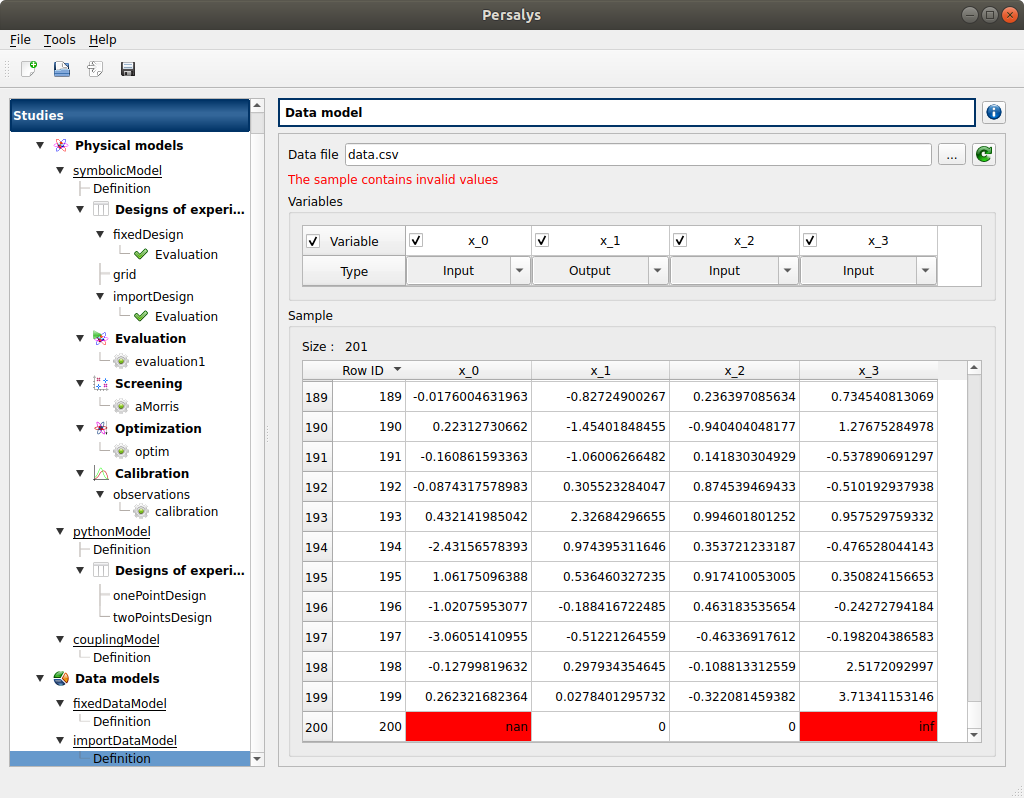
\includegraphics[height=0.65\textheight]{figures/cleaning1.png} 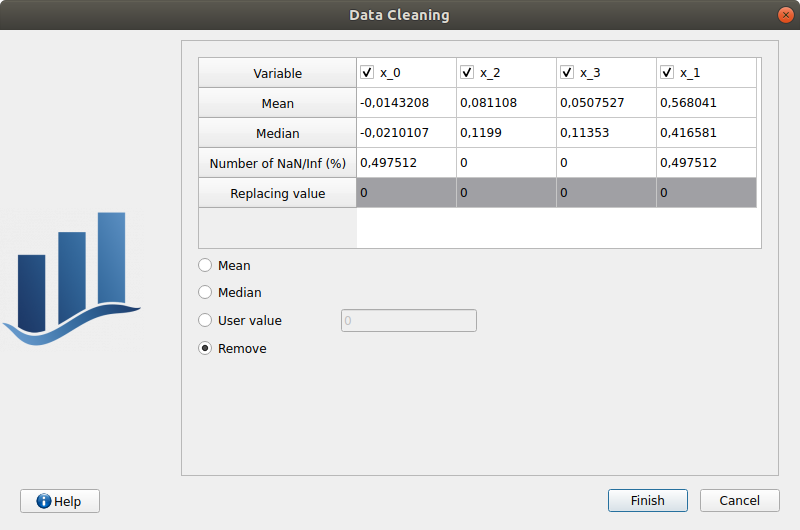
\includegraphics[height=0.65\textheight]{figures/cleaning2.png}
  \end{center}
\end{frame}

%%%%%%%%%%%%%%%%%%%%%%%%%%%%%%%%%%%%%%%%%%%%%%%%%%%%%%%%%%%%%%%%%%%%%%%%%%%%%

\begin{frame}
  \frametitle{Ergonomics - Python editor overhaul}
  \begin{itemize}
  \item Syntax highlighting and zooming in/out with ctrl+mouse-wheel
  \end{itemize}
  \begin{center}
    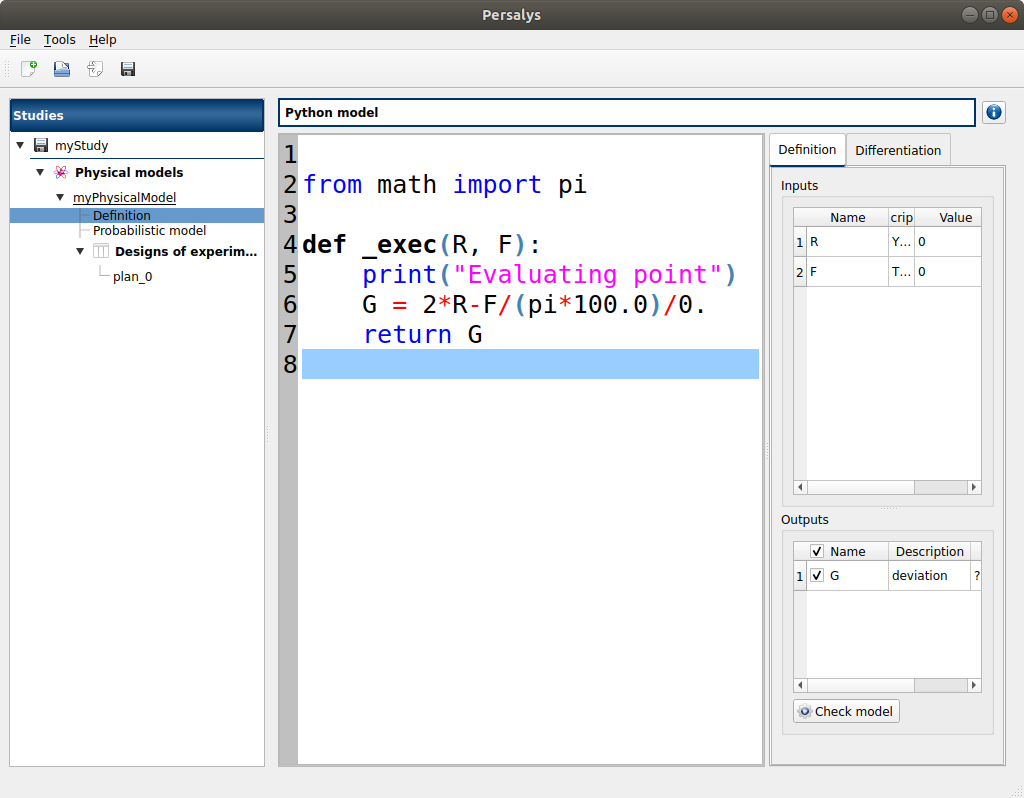
\includegraphics[height=0.65\textheight]{figures/python.png}
  \end{center}
\end{frame}

%%%%%%%%%%%%%%%%%%%%%%%%%%%%%%%%%%%%%%%%%%%%%%%%%%%%%%%%%%%%%%%%%%%%%%%%%%%%%

\begin{frame}
  \frametitle{Ergonomics - Optimization algorithms filters}
  \begin{itemize}
  \item Algorithms are filtered based on the problem definition (bounds, need for derivative)
  \item Link to algorithm documentation directly accessible
  \end{itemize}
  \begin{center}
    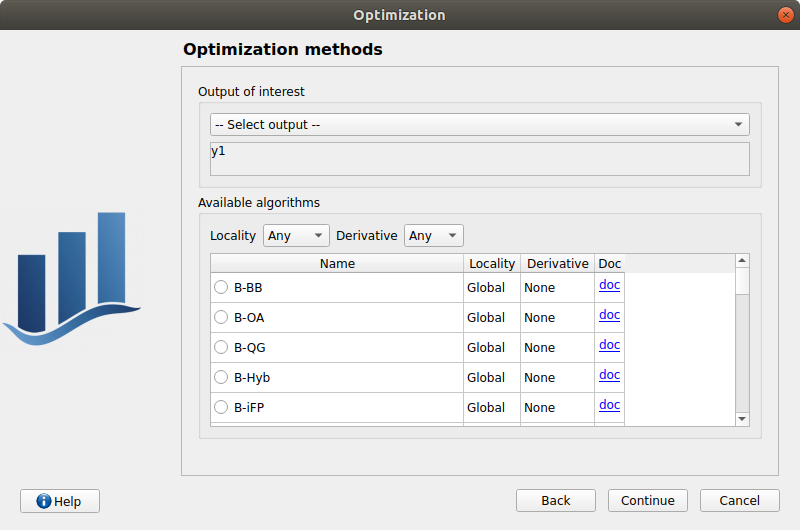
\includegraphics[height=0.65\textheight]{figures/optim.png}
 \end{center}
\end{frame}

%%%%%%%%%%%%%%%%%%%%%%%%%%%%%%%%%%%%%%%%%%%%%%%%%%%%%%%%%%%%%%%%%%%%%%%%%%%%%

\begin{frame}
  \frametitle{Ergonomics - DoE duration estimation - CSV import/export}
  \begin{itemize}
  \item Estimated DoE duration based on single evaluation
  \item CSV support improvements
    \begin{itemize}
    \item Numerical and column separator combinations are tested before importing data
    \item The user can choose numerical and column separator before exporting data
    \end{itemize}
  \end{itemize}
\end{frame}

%%%%%%%%%%%%%%%%%%%%%%%%%%%%%%%%%%%%%%%%%%%%%%%%%%%%%%%%%%%%%%%%%%%%%%%%%%%%%

\begin{frame}
  \frametitle{Coupling - Ansys coupling wizard (1)}
  \begin{itemize}
  \item Creating a coupling model can be tricky and/or tedious (command, resource, templates...)
  \item Added a wizard which helps the user to pre-fill the coupling model information
    \begin{itemize}
    \item The user specifies the workbench project and the blocks the will need updating
    \item The wizard looks for the Ansys solver based on project version
    \end{itemize}
  \end{itemize}
 \begin{center}
    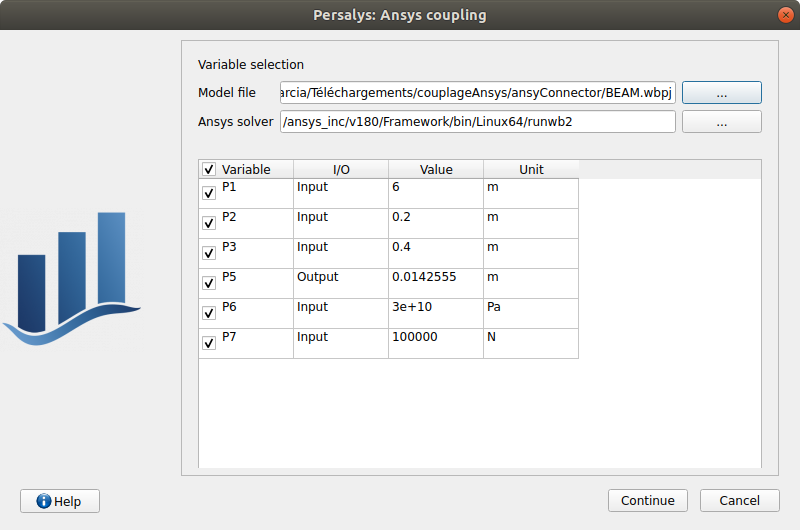
\includegraphics[height=0.6\textheight]{figures/ansys1.png}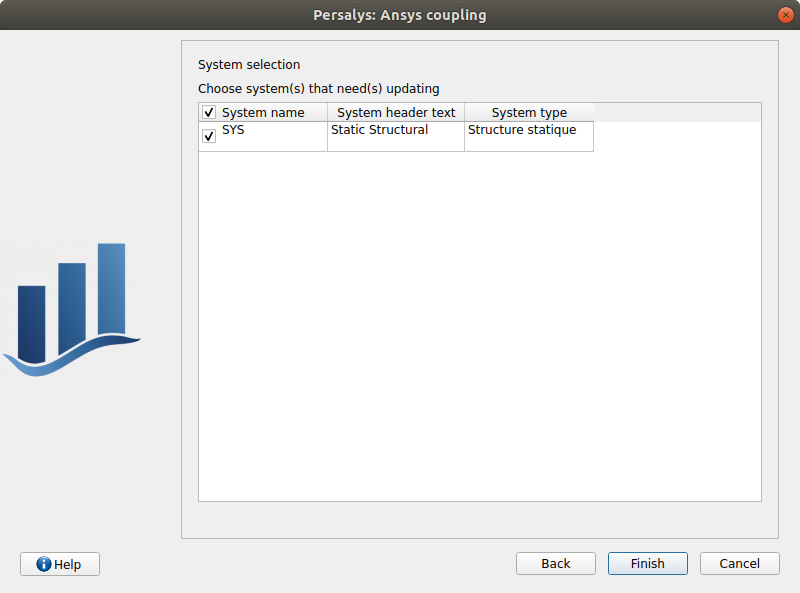
\includegraphics[height=0.6\textheight]{figures/ansys2.png}
 \end{center}
\end{frame}

%%%%%%%%%%%%%%%%%%%%%%%%%%%%%%%%%%%%%%%%%%%%%%%%%%%%%%%%%%%%%%%%%%%%%%%%%%%%%

\begin{frame}
\frametitle{Coupling - Ansys coupling wizard (2)}
  \begin{itemize}
  \item Input template file automatically generated based on variables selected by the user
  \end{itemize}
  \begin{center}
    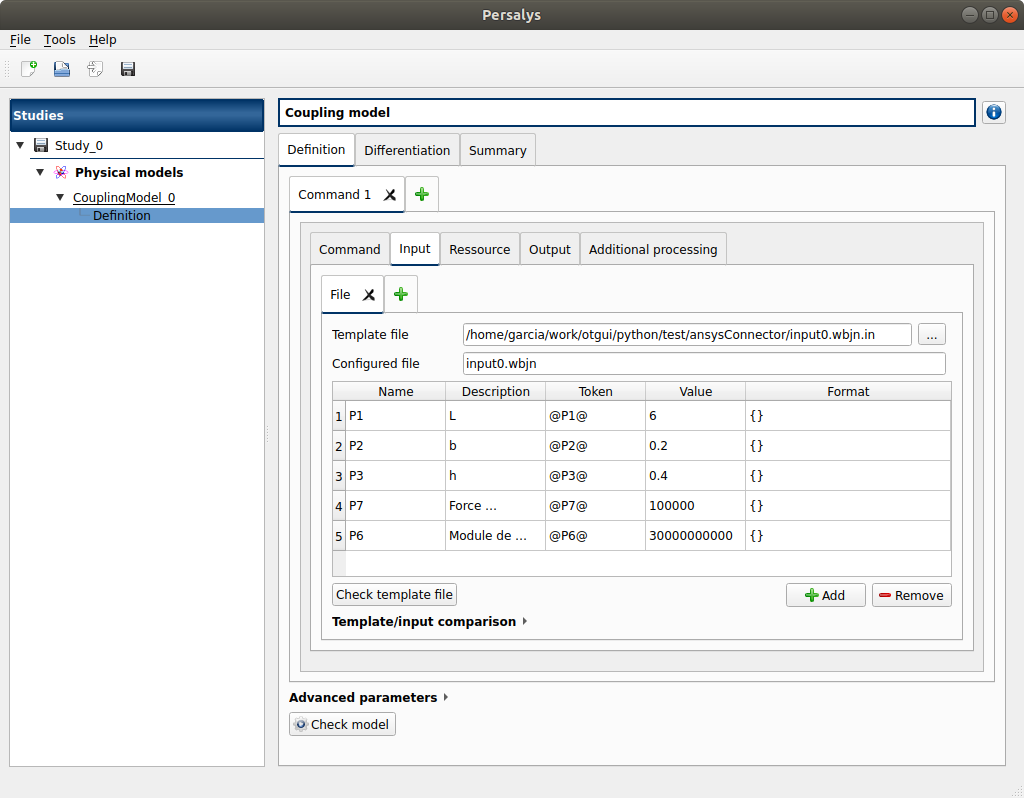
\includegraphics[height=0.6\textheight]{figures/ansys3.png}
  \end{center}
\end{frame}

%%%%%%%%%%%%%%%%%%%%%%%%%%%%%%%%%%%%%%%%%%%%%%%%%%%%%%%%%%%%%%%%%%%%%%%%%%%%%

\begin{frame}
  \frametitle{Coupling - Ansys coupling wizard (3)}
  \begin{itemize}
  \item Post processing step to account for Ansys output variables
  \end{itemize}
  \begin{center}
    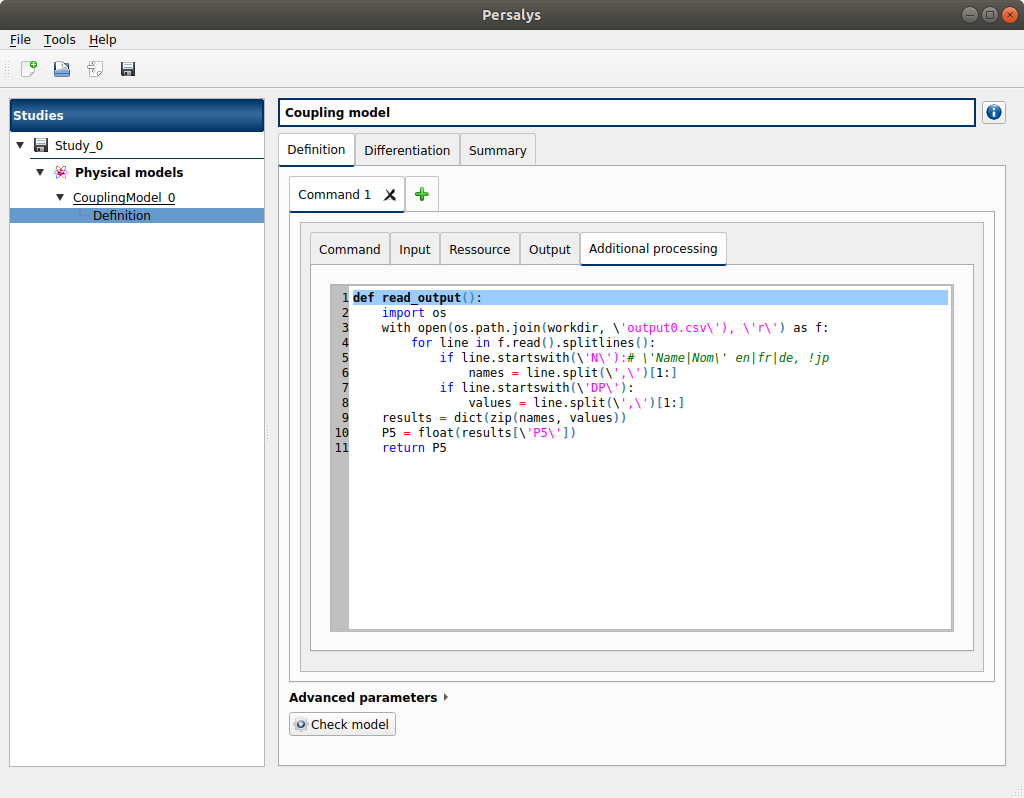
\includegraphics[height=0.6\textheight]{figures/ansys4.png}
  \end{center}
\end{frame}

%%%%%%%%%%%%%%%%%%%%%%%%%%%%%%%%%%%%%%%%%%%%%%%%%%%%%%%%%%%%%%%%%%%%%%%%%%%%%

\begin{frame}
  \frametitle{Coupling - Ansys coupling wizard (4)}
  \begin{itemize}
  \item Semi-automatic coupling model generation (everything is still modifiable by the user)
  \item Benefits from coupling model cache
    \begin{itemize}
    \item Already ran evaluation are skipped
    \item Failed points can be reran by editing the cache file
    \end{itemize}
  \end{itemize}
\end{frame}

%%%%%%%%%%%%%%%%%%%%%%%%%%%%%%%%%%%%%%%%%%%%%%%%%%%%%%%%%%%%%%%%%%%%%%%%%%%%%

\begin{frame}
  \frametitle{Features - HDF5 support}
  \begin{itemize}
  \item OpenTURNS updates allow to use \texttt{XMLH5StorageManager}
  \item Floats and integers are stored in HDF5 datasets (zip-like binary file)
  \item Speeds up studies writing/reading
  \item Saves up disk-space
  \end{itemize}
\end{frame}

%%%%%%%%%%%%%%%%%%%%%%%%%%%%%%%%%%%%%%%%%%%%%%%%%%%%%%%%%%%%%%%%%%%%%%%%%%%%%

\begin{frame}
  \frametitle{Features - Aggregated Sobol' Indices - Optimized LHS}
  \begin{itemize}
  \item Aggregated Sobol' Indices are now available for sensitivity analysis
  \item Optimizations for LHS : Simulated-annealing / Monte Carlo LHS available along with space filling algorithms
  \end{itemize}
  \begin{center}
    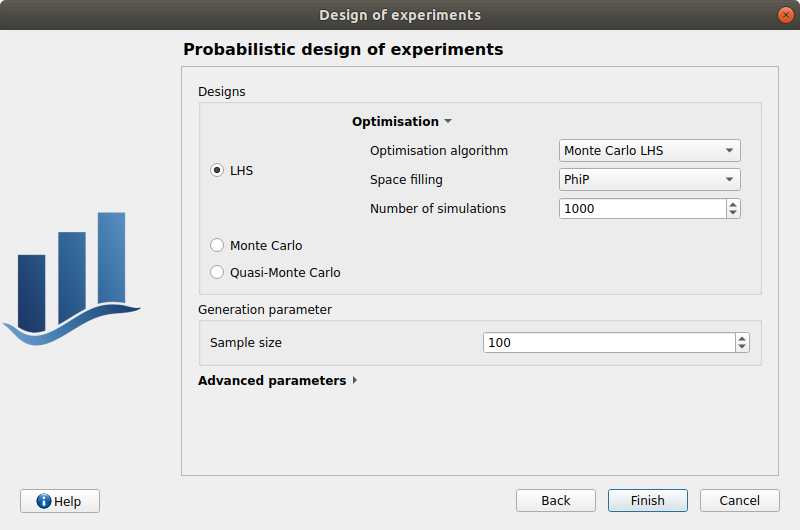
\includegraphics[height=0.6\textheight]{figures/LHS.png}
  \end{center}
\end{frame}

%%%%%%%%%%%%%%%%%%%%%%%%%%%%%%%%%%%%%%%%%%%%%%%%%%%%%%%%%%%%%%%%%%%%%%%%%%%%%

\section{What's next?}
\begin{frame}
\begin{small}


\begin{minipage}[t]{0.5\textwidth}
\underline{Field data (functional outputs)}
\begin{itemize}
\item 1D fields : better visualisation of large data sets
\item Import and analysis of field data sets
\item Handling of multi-dimensional fields (\textcolor{red}{long term developments})
\end{itemize}

\end{minipage}%
\begin{minipage}[t]{0.5\textwidth}
\underline{Linear regression implementation}
\begin{itemize}
\item Regression on polynomial bases of degrees 1 and 2
\item Optimal bases selection (step-wise method)
\item Validation \& results analysis (e.g., Cook distance, leverage)
\end{itemize}

\end{minipage}%

\vspace{12pt}

\begin{minipage}[t]{0.5\textwidth}
\underline{Handling of missing \& corrupted data}
\begin{itemize}
\item More robust identification of missing data
\item Alternative substitution methods
\item Better interactivity with data tables
\end{itemize}

\end{minipage}%
\begin{minipage}[t]{0.5\textwidth}
\underline{Exportation of surrogate models}
\begin{itemize}
\item Possibility of exporting the surrogate models created in Persalys in a python-compatible format easily usable in other scripts
\end{itemize}

\end{minipage}
\end{small}

\end{frame}



\begin{frame}
\begin{small}


\begin{minipage}[t]{0.5\textwidth}
\underline{Optimization}
\begin{itemize}
\item Handling of equality and inequality constraints
\item Implementation of heuristic (evolutionary) optimization algorithms
\item Possibility of solving multi-objective optimization problems
\end{itemize}

\end{minipage}%
\begin{minipage}[t]{0.5\textwidth}
\underline{Ergonomic improvements}
\begin{itemize}
\item Paraview : better visualisation and interactivity
\item Physical models : numerical differentiation parametrization made more visible
\end{itemize}

\end{minipage}

\vspace{12pt}

\begin{minipage}[t]{0.5\textwidth}
\underline{Kriging}
\begin{itemize}
\item Possibility of performing multi-start optimization when training the model
\end{itemize}

\end{minipage}%
\begin{minipage}[t]{0.5\textwidth}
\underline{Computation on servers}
\begin{itemize}
\item Possibility of stop and restart analyses, even when performed on servers
\item Better handling of error logs
\end{itemize}
\end{minipage}
\end{small}
\end{frame}



\begin{frame}
\frametitle{The end}
\begin{center}
Thanks !
\end{center}

\begin{center}
Questions ?
\end{center}

\end{frame}

\note{
Thank you for your attention.

If you have any question, it would be a pleasure to answer them.

If you want a live demo of PERSALYS, I can show you during the coffee break.
}

% %%%%%%%%%%%%%%%%%%%%%%%%%%%%%%%%%%%%%%%%%%%%%%%%%%%%%%%%%%%%%%%%%%%%%%%%%%%%%

\end{document}
